\chapter{Analyse}

\section{Einordnung des Kreditorenworkflows}
Um die Intention der Neukonzeption verstehen und sie angemessen durchführen zu können, wird der Prozess zunächst im Unternehmen eingeordnet.\footnote{Die ISO 9001 fordert z.B. in Kapitel 4.2.2 zur Qualitätssicherung in Prozessen ein Verständnis der Abhängigkeiten und Wechselwirkungen dieser. Frameworks wie ITIL oder die Six Sigma Methode nutzen ebenfalls Prozessportfolios im Rahmen von Einführung, Management und Optimierung.}\\
%Die Einordnung in das Prozessportfolio kann z.B. auf Grundlage von Six Sigma erfolgen.
Dazu werden die strategische Relevanz (bzw. Bedeutung für den Geschäftserfolg) und der Verbesserungsbedarf gegenübergestellt. 
Diese Gegenüberstellung erfolgt qualitativ und auf Basis der Einschätzung von Mitarbeitern des Managements (Bereichsleiter, Vorstand).
Je  Dimension sind mehrere Kriterien (Strategische Bedeutung: Marktrelevanz, Geschäftskritikalität, Marktfähigkeit; Verbesserungsfähigkeit: Technologische Unterstützung, Fehleranfälligkeit, Performance) zu bewerten. 
Das Mittel aller Einschätzungen ergibt die Positionierung im Portfolio-Diagramm.

\begin{figure}[!htb]
\centering
\includegraphics[height=60mm]{images/portfolio}
\caption{Portfolioeinordnung des Kreditorenworkflows \protect\footnotemark}
\label{Portfolioeinordnung des Kreditorenworkflows}
\end{figure}
\footnotetext{Quelle: Autor}

Es ergibt sich ein hohes Verbesserungspotential, dessen Erläuterung Teil dieses Kapitels ist.
Die ebenfalls hohe strategische Relevanz resultiert aus zwei Rahmenbedingungen. 
Zum einen ist die Rechnungslegung gegenüber dem Gesetzgeber verpflichtend und ist daher für den Geschäftsbetrieb unerlässlich. 
%Dieser Umstand sorgt jedoch nicht allein für die Einordnung. 
Entscheidend ist aber, dass die Kreditorenbuchhaltung auch als Service von der \firma angeboten wird.
Das bedeutet konkret, dass Firmen (insbesondere Beteiligungsfirmen, also Bestandteile der GLC Group) die Kreditorenbuchhaltung an die \firma  outsourcen können. 
Dementsprechend wird in dem Prozess auch fakturierbarer Service gegenüber Kunden generiert.\\
Ordnet man nun diesen Prozess in eine Prozesslandkarte ein, wie im Rahmen von ISO 9000 beispielsweise gängig, ein, zeigt sich, dass der Prozess nicht ausschließlich, wie bei Inhalten der Finanzbuchhaltung ansonsten üblich, als Unterstützungsprozess einzustufen ist.\\
\begin{figure}[!htb]
\centering
\includegraphics[height=60mm]{images/prozesslandkarte}
\caption{Portfolioeinordnung des Kreditorenworkflows \protect\footnotemark}
\label{Portfolioeinordnung des Kreditorenworkflows}
\end{figure}
\footnotetext{Quelle: Autor}
~\ \\Vielmehr zeigt sich, dass, je nach Prozessinstanz, eine Einordnung als Kernprozess (bzw. Leistungsprozess) oder Unterstützungsprozess (bzw. Supportprozess) möglich ist. 
Mehrheitlich betreffen die Prozessinstanzen interne Rechnungen, welche als Supportprozess eingeordnet werden. \\
Hinsichtlich Kundenrechnungen, welche eher Leistungsprozessinstanzen darstellen, ergeben sich jedoch teilweise differierende Anforderungen an den Prozess.
Dieser Umstand wird im weiteren Verlauf berücksichtigt.


\section{Ist-Aufnahme}
Der Prozess wird in zwei sequentiellen Stufen betrachtet. 
Im ersten Teil geht die Rechnung  ein und wird freigegeben.
Im zweiten Teil wird die Rechnung gebucht und der Zahllauf vorbereitet.
Diese Trennung ergibt sich vor allem aus dem Grad der technologischen Unterstützung, welcher zwischen diesen Teilprozessen deutlich differiert.
\subsection{Kreditorenworkflow Teil 1: Rechnungsfreigabe}
Der erste Teil beginnt streng genommen mit der Kostenverursachung, auf die eine Kreditorenrechnung folgt. 
Da die Durchführung der Kostenverursachung selbst allerdings für den Workflow nicht weiter relevant ist (sie erfolgt losgelöst), wird der Rechnungseingang als Ausgangspunkt des Prozesses und Auslöser einer Prozessinstanz betrachtet. 
\subsubsection{Prozessablauf}
Die eingehende Kreditorenrechnung wird innerhalb des Unternehmens an einen bestimmten Mitarbeiter der Finanzbuchhaltung gegeben (Kreditorenbuchhaltung in der Regel mit einer Person besetzt).
Dieser setzt zum einen einen Stempel auf die Rechnung für das Eingangsdatum.
Zum anderen wird der Buchungsstempel gesetzt, der die Eintragung buchungsrelevanter Daten ermöglicht bzw. später einfordert (Kostenstelle, Kostenträger/Projektnummer, sachliche Freigabe, fachliche Freigabe, Infos).\\
Für die nachfolgenden Schritte gibt es zwei mögliche Szenarien.

\paragraph{Fall 1: Kostenverursacher in Niederlassung}
~\\ 
In diesem Szenario befindet sich der Kostenverursacher nicht in der Unternehmenszentrale, sondern in räumlicher Distanz zur Finanzbuchhaltung.\\
Der Mitarbeiter scannt die Rechnung ein (erster Schritt der Versionierung). $\rightarrow$
Danach muss die Rechnung zur sachlichen Freigabe an den Kostenverursacher gesendet werden, dies geschieht in der Regel per E-Mail mit dem angehängten Scan des Originals.
Wird die Rechnung sachlich nicht freigegegeben, endet die Prozessinstanz.
Nachfolgend müssen vom Mitarbeiter der Finanzbuchhaltung die Gründe dafür eruiert und ggf. eine korrekte Rechnung nachgefordert werden.$\rightarrow$
Soll die Rechnung sachlich freigegeben werden, druckt der freigebende Mitarbeiter dazu die Rechnung aus, unterschreibt im Buchungsstempel und scannt das Resultat wieder.
Dieses sendet er dem Mitarbeiter der Finanzbuchhaltung per E-Mail zurück.
Der Mitarbeiter druckt wiederum das die sachlich freigegebene Rechnung aus.
Danach muss die fachliche Freigabe erfolgen.
Dazu verbringt der Mitarbeiter die Original-Rechnung und den Ausdruck mit der sachlichen Freizeichnung an den verantwortlichen Bereichsleiter.
Dieser lehnt ggf. die Rechnung ab, dazu wird wie im Fall der sachlichen Freigabe verfahren.
Im Regelfall gibt er mit seiner Unterschrift die Rechnung fachlich frei und trägt Kostenstelle und (Projekt-)Kostenträger ein.
Ggf. erfolgt ein Vermerk, dass die Rechnung an einen Kunden weiterzuberechnen ist (Im ''Infos''-Feld des Buchungsstempels). 
Nachdem die fachliche Freigabe erfolgt ist, wird die finale Version eingescannt.\\
Damit liegen alle Freigaben vor und der Mitarbeiter ist zur Buchung berechtigt.

\paragraph{Fall 2: Kostenverursacher in Unternehmenszentrale}
~\\
In diesem Szenario befindet sich der Kostenverursacher in der Unternehmenszentrale, also in für die Mitarbeiter der Finanzbuchhaltung erreichbarer Nähe.
Zunächst muss ebenso die sachliche Freigabe erfolgen.
Dazu verbringt der Mitarbeiter der Finanzbuchhaltung die Original-Rechnung an den Kostenverursacher.
Für eine nicht erfolgende Freigabe wird wie Fall 1 beschrieben verfahren.
Erfolgt die sachliche Freigabe (Unterschrift im Buchungsstempel), hat wie im ersten Fall als nächstes die fachliche Freigabe zu erfolgen.
Dazu wird ebenfalls die Original-Rechnung, diesmal allerdings mit sachlicher Freigabe an den Bereichsverantwortlichen verbracht.
Im Regelfall gibt er mit seiner Unterschrift die Rechnung fachlich frei.
Ggf. erfolgt auch hier ein Vermerk, der die Weiterberechnung anweist.
Für nicht erfolgende fachliche Freigabe wird erneut wie beschrieben verfahren (verwerfen, ggf. Rechnung nachfordern)
Danach gibt der mit der sachlichen Freigabe beauftragte Mitarbeiter die Belege über die interne Post zurück an die Finanzbuchhaltung.
Dort wird abschließend die vollständig freigezeichnete Version eingescannt.
Damit liegen alle Freigaben vor und der Mitarbeiter ist zur Buchung berechtigt.

\subsubsection{Prozessmodellierung}
Der Prozess lässt sich prinzipiell für beide Fälle einheitlich modellieren, da der inhaltliche Ablauf (Freigabe-Sequenz) identisch ist.
Der wesentliche Unterschied zwischen diesen möglichen Prozessverläufen ist lediglich eine Erhöhung des Papieraufkommens durch die Kombination von Scan, Versendung und Druck.\\
Zu beachten ist, dass der Prozess Schnittstellen aufweist.
Eine davon ist die zur Debitorenbuchhaltung, die bei einem Weiterberechnungsvermerk greift. 
%Diese wird modelliert, ist allerdings inhaltlich in diesem Rahmen nicht relevant.
Die zweite Schnittstelle ist die Verbindung zum zweiten Teil des Workflows.\\

%Im Anhang muss das nochmal im Detail sein

\begin{figure}[!htb]
\centering
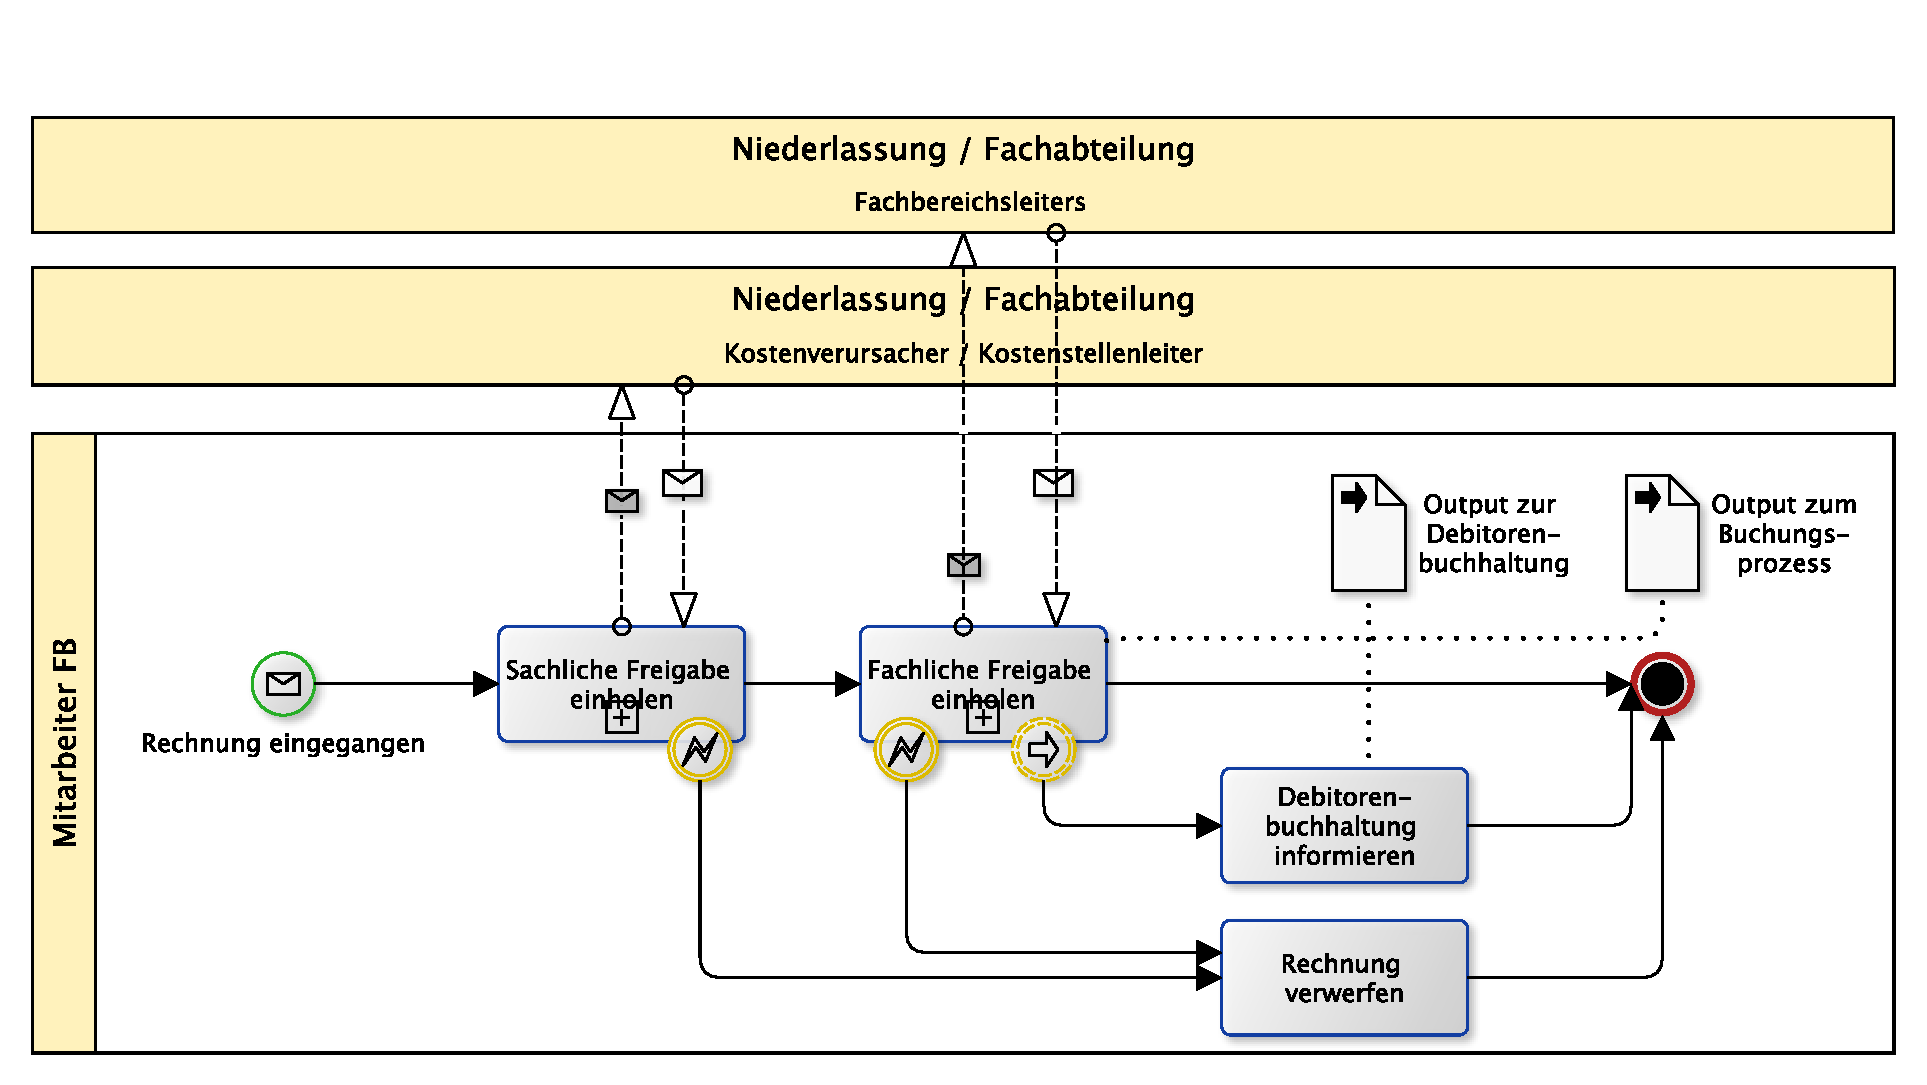
\includegraphics[height=85mm]{images/Prozess_Ist_1_Simpel.pdf}
\caption[Teilprozess 1 im Ist-Zustand, BPMN simpel]{Der erste Teilprozess im Ist-Zustand \protect\footnotemark}
\label{Teilprozess 1 im Ist-Zustand, BPMN simpel}
\end{figure}
\footnotetext{Quelle: Autor}

\subsection{Kreditorenworkflow Teil 2: Rechnungsbuchung}
Während der erste Teil nur provisorisch durch IT-Systeme gestützt wird (pragmatische Verwendung von E-Mails), werden im zweiten Teil zur Buchung bereits Bestands-EDV-Systeme benutzt.
\subsubsection{Prozessablauf}
Zur Buchung müssen die Rechnung, die Freigaben (sachlich und fachlich) sowie die Informationen der Kostenempfänger (Kostenstelle und (Projekt-)Kostenträger) vorliegen.
Dann werden alle im Laufe der Freigabe entstandenen Belegversionen digital an Datev Rechnungswesen Pro übergeben.
Das Feature der automatischen Zeichenerkennung erkennt dabei insbesondere die Rechnungsnummer, das Rechnungsatum, den Saldo und die Steuer.
Die Kostenstelle, sowie der Kostenträger müssen durch den Mitarbeiter manuell angegeben werden.
In Datev wird die Rechnung dem Kreditor und unter diesem wiederum der Rechnungsnummer zugeordnet.
Damit ist die Rechnung in Datev verbucht.\\
Die Rechnung muss anschließend noch gezahlt werden.\\
Dazu wird regelmäßig (im Normalfall wöchentlich) ein Zahllauf in Datev angelegt.
In diesem erscheinen die fälligen Belege. 
Die Fälligkeit ergibt sich hierbei aus Rechnungsdatum und Zahlungsziel, welches aus den Kreditorenstammdaten entnommen wird.
Die fälligen Zahlungen werden nun zunächst durch den Mitarbeiter selbst geprüft.
Anschließend wird der Zahllauf dem Vorstandsvorsitzenden in Schriftform zur Freigabe vorgelegt.
Ist die Freigabe erfolgt, werden die Zahlungsanweisungen in einer Datei an das eBanking-System gegeben.
Ein zweiter Mitarbeiter prüft die Freigabe durch den Vorstandsvorsitzenden und gibt die Zahlungen im eBanking-System frei.
Das eBanking-System übermittelt daraufhin die Zahlungen an die Bank, wo die Zahlung durchgeführt wird.
\subsubsection{Prozessmodellierung}

Auch dieser Teilprozess lässt sich mit dem gegebenen Ablauf modellieren. 
Die Durchführung der Zahlung kann als transparent betrachtet werden, da sie vollautomatisch durchgeführt wird.


\begin{figure}[!htb]
\centering
\includegraphics[height=90mm]{images/Prozess_ist_buchung.pdf}
\caption[Teilprozess 2 im Ist-Zustand, BPMN]{Der zweite Teilprozess im Ist-Zustand \protect\footnotemark}
\label{Teilprozess 2 im Ist-Zustand, BPMN}
\end{figure}
\footnotetext{Quelle: Autor}
\newpage


\section{Problemanalyse}


\subsection{Methodik der Problemanalyse}

%\begin{wrapfigure}{r}{0.4\textwidth}
 % \begin{center}
 %   \includegraphics[width=0.38\textwidth]{images/problemanalyse}
 % \end{center}
 % \caption{Verlauf der Problemanalyse}
%\end{wrapfigure}
Die nun folgende Problemanalyse ist Ausgangspunkt für die Neukonzeption.
%Zur Identifikation von problematischen Aspekten wird zunächst die argumentative Grundlage aufgezeigt, auf Basis derer die Probleme erläutert werden.\\
Die Analyse wird in zwei Teilen durchgeführt.
Einerseits dienen dazu Interviews mit Prozessbeteiligten. 
Diese werden mittels Stakeholderanalyse identifiziert.\\
Mittels der Interviews werden Fehlerquellen und -arten identifiert, außerdem wird die wahrgenommene Prozessperformance ausgewertet und in KPIs überführt, anhand dener sie gemessen werden kann.\\
Ferner werden die Prozessbeschreibungen bzw. Prozessmodelle ausgewertet.
Aufgrund dieser werden Ansätze zur Verbesserung herausgearbeitet.

\subsection{Stakeholderanalyse}
Die Stakeholder des Prozesses ergeben sich aus den Akteuren, die in der Prozessbeschreibung bzw. der Prozessmodellierung als Beteiligte auftreten.\\
Das sind:


\begin{enumerate}
\item{Mitarbeiter der Finanzbuchhaltung}
\\ Speziell der Mitarbeiter der Finanzbuchhaltung, der für die Kreditorenbuchhaltung zuständig ist, ist in diesem Rahmen aktiv. 
\\ Ein weiterer Akteur aus diesem Bereich ist der (faktisch wechselnde) Mitarbeiter, der den Zahllauf nach dem Vieraugen-Prinzip freigibt. 
Dieser ist jedoch nur marginal beteiligt.
\\ Ein Stakholder, obgleich nicht maßgeblich am Prozessablauf beteiligt, ist der Leiter der Finanzbuchhaltung, der die Prozesse der Abteilung plant, deren Implementation steuert und den Ablauf kontrolliert.

\item{Kostenstellenverantwortliche}
\\ Die Kostenverursacher sind Mitarbeiter, die zur Kostenverursachung befugt sind. 
Faktisch sind dies Kostenstellenverantwortliche, die regelmäßige oder abwicklungsbezogene Kosten verursachen und damit Kreditorenrechnungen auslösen. 
Durch sie erfolgt die sachliche Freigabe.

\item{EDV-Abteilung}
\\ Da der Prozess teilweise technologiegestützt abläuft, ist die Abteilung der Informationstechnologie, wenn auch nicht aktiv an Prozessinstanzen beteiligt, als Stakeholder auszumachen. 

\item{Bereichsverantwortliche}
\\ Die Mitarbeiter, die die fachliche Freigabe erteilen dürfen, sind Bereichsleiter. 
Konkret lässt sich dies zum Zeitpunkt der Erstellung dieser Arbeit auf drei Personen konkretisieren. 
Von diesen befinden sich zwei im Vorstand, der dritte ist der Bereichsleiter Informationstechnologie.

\end{enumerate}
~\ \\
Aus dieser Liste lassen sich konkrete Personen ableiten, deren Erfahrung mit dem Prozess zur Problemidentifikation dienen kann. 
Mit diesen werden Interviews geführt, um eine empirische Grundlage zu schaffen.

Es ergeben sich:

\begin{enumerate}
\item{Mitarbeiter der (Kreditoren-)Buchhaltung}
\item{Leiter der Finanzbuchhaltung}
\item{Ein Bereichsverantwortlicher}
\item{Leiter der Informationstechnologie}
\end{enumerate}

\subsection{Interviewkonzeption}
Mit den erläuterten Stakeholdern werden Interviews geführt.
In diesen werden die Kernpunkte zur Identifikation von Prozessschwachstellen abgedeckt, welche werden in zwei Bereiche aufgeteilt sind.


\begin{table}[!htb]
\centering
\caption{Fragenkategorien des Interviewbogens}
\label{Fragenkategorien des Interviewbogens}
\begin{tabular}{|p{8cm}|p{8cm}|}
\hline
\rowcolor[HTML]{FFFFC7} 
{\color[HTML]{000000} \textbf{Fehler}} & {\color[HTML]{000000} \textbf{Sonstige Schwachstellen}} \\ \hline
\textbf{Fehlerarten} - \newline Welche Fehlervarianten treten auf?   &  \textbf{Prozessperformance} - \newline Woran bemisst sich die Performance des Prozesses? \newline                           \\ 
\textbf{Fehlerhäufigkeit} - \newline Wie häufig treten Fehler auf?  &   ~\ \newline Wie ist die Performance des Prozesses generell zu beurteilen?   \newline     ~\                                                                      \\ 
\textbf{Fehlerquellen} - \newline Welche Fehlerquellen sind ersichtlich? & \textbf{Performanceschwächen} - \newline Welche Gründe gibt es für suboptimale Performance?  \\                            

\hline
\end{tabular}
\end{table}


\subsection{Auswertung Interviews}






\subsubsection{Fehler}
Eine von zwei Möglichkeiten, die im Zusammenhang mit dem Prozess problematisch sind, sind fehlerhafte Prozessinstanzen. Als fehlerhaft wird eine Prozessinstanz betrachtet, wenn diese nicht wie beschrieben abläuft, also der Modellierung nicht folgt.

\paragraph{Fehlerarten}\label{fehlerarten}
~\ \\
Die genannten Fehler lassen sich sich in zwei Kategorien zusammenfassen.

\begin{enumerate}
\item{Rechnung nicht zugegen}
\\ Die Rechnung befindet sich zu einem bestimmten Zeitpunkt nicht am vorgesehenen Ort. 
Sie ist entweder nicht in die Finanzbuchhaltung gegeben worden oder auf sonstige Art auf dem Weg des Freigabeprozesses verloren gegangen.
\item{Formal nicht korrekte Rechnung}
\\ Die Rechnung weist nicht alle Daten auf, die zur sachlichen und fachlichen Freigabe ggf. nötig wären, sodass Rücksprache mit dem Kreditor notwendig ist.
\end{enumerate}


\paragraph{Fehlerquellen}
~\ \\
Für die festgestellten Fehler werden von den Stakeholdern konkrete Fehlerquellen verantwortlich gemacht.
Die bereitgestellten Systeme werden im Rahmen des Nutzungsbereichs als adäquat und funktional betrachtet.
Als problematisch wird nur der Teil empfunden, in dem keine IT-System-seitige Prozessunterstützung stattfindet.
Die Gründe für fehlerhafte Prozessinstanzen sind demnach auf menschliches Verhalten zurückzuführen, welches in diesem Zusammenhang durch Nachlässigkeit die beschrieben Fehler auslöst.
\\
Bezüglich fehlerhafter Rechnungen ist die Ursache meistens auf Nachlässigkeit seitens des Kreditors zurückzuführen.
Da diese von internen Prozessen losgelöst ist, steht diese Fehlerquelle nicht im Fokus dieser Arbeit. 

\subsubsection{Performance}\label{performance}
Die zweite Möglichkeit für eine als problematisch wahrgenommene Prozessinstanz ist deren mangelhafte Performance.
Diesbezüglich gibt es mehrere Anhaltspunkte, die von Stakeholdern angesprochen werden.
Zum einen gestalten sich Prozessdurchläufe langwierig.
Unabhängig davon, ob die Freizeichnung mit Akteuren durchgeführt wird, die sich inner- oder außerhalb der Unternehmenszentrale befinden und dementsprechend eine räumliche Entfernung zwischen der Finanzbuchhaltung und den Freizeichnern ergibt vorliegt oder nicht, ist der Freigabeprozess mit hohem manuellen Kommunikationsaufwand verbunden, der über E-Mail oder direkt, allerdings mit Laufwegen durch das Unternehmen bearbeitet wird.
\\
Aus diesem Umstand ergibt sich auch die mangelhafte Kontrollmöglichkeit, sowohl für den betroffenen Mitarbeiter der Finanzbuchhaltung, als auch die mit der Freizeichnung beauftragten Akteure, da sich Rechnungen in der zu einem bestimmten Zeitpunkt aktuellen Version faktisch nur im Zugriff eines einzelnen Mitarbeiters befinden. 
Besonders deutlich wird diese Situation bei Rechnungen, die innerhalb der Unternehmenszentrale durchgereicht werden.
An jeder Station (also Rechnungsannahme, sachliche Freigabe, fachliche Freigabe und wieder zurück in der Finanzbuchhaltung) besteht zusätzlich die Möglichkeit, dass ein Beleg abhanden kommt und eine neue Prozessinstanz erst durch Nachsendung einer Mahnung oder Zahlungserinnerung ausgelöst wird.

\paragraph{Key Performance Indicators}
~\ \\
Diese Kritikpunkte lassen sich in objektiven Kennzahlen ausdrücken, an denen die Prozessqualität im Ist-Zustand gemessen werden kann. 
Diese sollen auch die Neukonzeption des Prozesses begleiten, bzw. diese an der Verbesserung resultierender Werte ausgerichtet werden.
Auf Basis der Erläuterungen in \ref{fehlerarten} und \ref{performance} ergeben sich zwei Kennzahlen:

\begin{enumerate}
\item{Prozesslaufzeit}
\\ Die objektiv messbare Zeit von Rechnungseingang/-annahme bis Bezahlung, speziell jedoch in dem als performanceschwach wahrgenommenen Teil von Rechnungseingang/-annahme bis Buchung.
\item{Prozessfehlerrate}
\\ Relativer Anteil fehlerhafter Prozessinstanzen.
\end{enumerate}



\subsection{Auswertung des Prozessablaufs}
Die Teilprozesse können separat ausgewertet werden.\\
Der inhaltliche Ablauf der Rechnungsfreigabe ist relativ simpel.
Die Freigabe findet nach dem Vieraugenprinzip in einem annähernd statischen Prozess statt, sprich: es sind nur minimal variable Prozessverläufe möglich, da es kaum Entscheidungsmöglichkeiten (Gateways in BPMN) gibt.
Unterschiedliche Verläufe sind nur möglich, wenn die Rechnung an einer Stelle abgelehnt wird.\\
Auffälligkeiten ergeben sich in den Details des Ablaufes: 
Auffällig ist primär, dass der gesamte Belegverkehr vor der Buchung händisch erledigt wird. 
Es findet keine zentrale Versionsverwaltung statt (im Falle einer Versendung per Mail liegen alle Versionen in den Postfächern der betroffenen Mitarbeiter).
Dieser Ablauf bietet keinerlei externe Nachvollziehbarkeitsmöglichkeiten.
Um effektiv kontrollieren zu können, müsste ein Dritter in jeden Prozessschritt involviert werden oder die Postfächer aller in Frage kommenden Personen überwachen.
Hinzukommt, dass dadurch Belege verloren gehen können.
Dies gilt insbesondere für die sachliche Freigabe.
Die fachliche Freigabe wird im Regelfall nicht per E-Mail-Verkehr erledigt, da alle Bereichsleiter in der Unternehmenszentrale ansässig sind. 
In diesem Fall ergibt sich jedoch, wie ansonsten für die sachliche Freigabe ebenfalls, die Problematik intern überreichter Belege.
In dieser Konstellation ergibt sich jedoch insofern dieselbe prinzipielle Schwierigkeit, als hierbei zwar keine Isolation der Belegversionen in Postfächern stattfindet, aber die Originale nicht verfolgbar durch die Unternehmenszentrale gereicht werden.
\\[1\baselineskip]
Der zweite Teilprozess (Buchung und Bezahlung) läuft ähnlich gut kalkulierbar wie der erste Teilprozess ab.
Lediglich die Zahlungsfreigabe des Vorstandsvorsitzenden ist ein Faktor, der den Verlauf einer Prozessinstanz beeinflussen kann. 
Lehnt dieser z.B. eine einzelne Zahlung eines Zahllaufes vorübergehend ab, weil er eine fakturierte Leistung als nicht final erbracht wertet, muss der Mitarbeiter der Kreditorenbuchhaltung diese Zahlung aus dem anstehenden Zahllauf entfernen.
Diese bleibt aber bis zur abschließenden Zahlung als fällig markiert und ist im nächsten Zahllauf erneut inkludiert.
Zwar findet auch in diesem Teilprozess manueller Belegverkehr statt, dieser ist aber insofern reproduzierbar, als dafür bereits gebuchte Belege aus Datev genutzt werden. 
Dementsprechend kann in diesem Szenario kein Beleg in Vergessenheit geraten.
Entscheidend ist, dass dieser Teilprozess durch davor vorgesehene IT-Systeme gestützt wird.
Die Erkenntnisse aus den Interviews decken sich mit dieser Einschätzung.
Teilweise wird wird dieser Vorgang als nicht verbesserungsfähig bzw. -würdig betrachtet.



